\chapter{Wprowadzenie} \label{ch:wprowadzenie}

Choroba Parkinsona (ang. \emph {Parkinson Disease, PD}) to zwyrodnieniowe schorzenie mózgu, które wiąże się z objawami ruchowymi, takimi jak spowolnienie ruchowe,
drżenie, sztywność oraz zaburzenia chodu i równowagi.
Ponadto może prowadzić do różnorodnych powikłań niemotorycznych, obejmujących zaburzenia poznawcze, stany psychiczne,
trudności ze snem oraz dolegliwości sensoryczne, w tym ból.
Początkowe objawy często rozwijają się stopniowo, nasilając się w miarę upływu czasu.
Postęp choroby prowadzi do znacznego stopnia niepełnosprawności, co może wymagać wsparcia i opieki.

\begin{figure}[htbp]
	\centering
	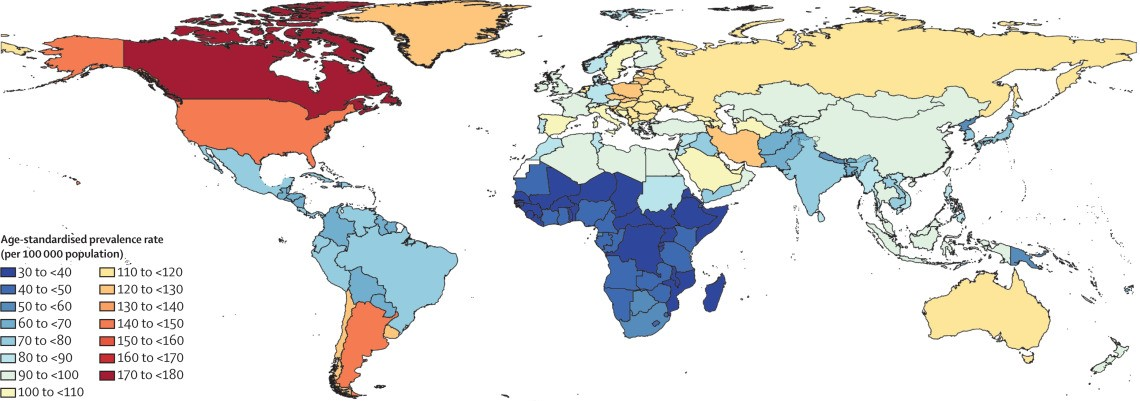
\includegraphics[width=0.9\textwidth]{./img/map}
	\caption{Choroba Parkinsona na świecie~\cite {global_PD}}
    \label{fig:PD_map}
\end{figure}

Zgodnie z danymi przedstawionymi w raporcie Światowej Organizacji Zdrowia~\cite{WHO}, choroba Parkinsona stanowi obecnie narastający problem na skalę światową.
Zarówno wskaźniki niepełnosprawności, jak i zgony związane z tą chorobą rosną szybciej niż w przypadku innych zaburzeń neurologicznych.

W ciągu ostatnich 25 lat zaobserwowano podwojenie częstości występowania PD na całym świecie.
Globalne szacunki na rok 2019 wskazują, że liczba osób cierpiących na PD przekroczyła 8,5 miliona, co oznacza wzrost o 81\% w porównaniu z danymi z roku 2000.
Jednocześnie liczba zgonów związanych z PD wyniosła 329~000, co stanowi wzrost o ponad 100\% w porównaniu z rokiem 2000~\cite{global_PD}.
W Polsce z chorobą tą zmaga się około 100 tys.
pacjentów, z czego około 20\% jest już w stadium zaawansowanym
według informacji przekazywanych przez Fundację Chorób Mózgu.
Ponadto co roku w naszym kraju wykrywanych jest ok.
8 tys.
nowych zachorowań.

PD jest istotną sprawą dotyczącą zdrowia publicznego, ponieważ jej częstotliwość występowania związana jest ze zjawiskiem starzejącego się społeczeństwa (Rys.~\ref{fig:PD_map}).
Razem z innymi chorobami neurodegeneracyjnymi, takimi jak choroba Alzheimera, ma szanse stać się drugą zaraz za nowotworami przyczyną zgonów do 2040 roku (WHO).

\begin{figure}[htbp]
	\centering
	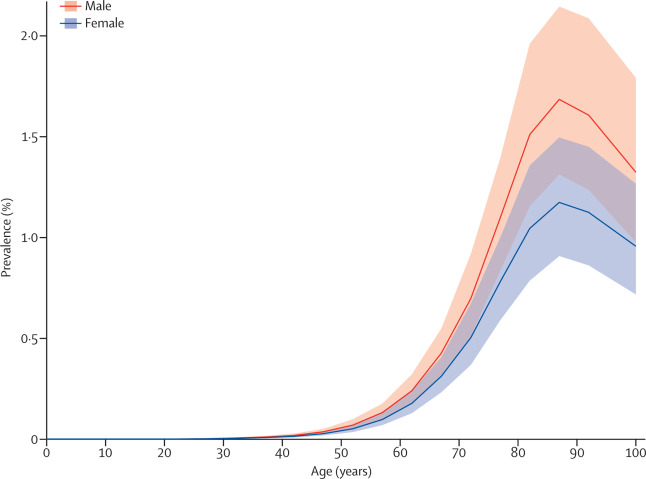
\includegraphics[width=0.6\textwidth]{./img/PD_prevalence}
	\caption{Rozpowszechnienie choroby Parkinsona w zależności od wieku \cite {global_PD}}
    \label{fig:PD_prevalance}
\end{figure}

Każdy może być narażony na ryzyko rozwoju choroby Parkinsona, ale częściej występuje ona u mężczyzn niż u kobiet (Rys.\ref{fig:PD_prevalance}).
Statystyki pokazują, że ryzyko zachorowania rośnie wraz z wiekiem, chociaż może ona dotyczyć także młodszych osób (nawet w wieku 20 lat).
U większości pacjentów po raz pierwszy choroba rozwija się po 60 roku życia, około 5\% do 10\% doświadcza jej początku przed 50 rokiem życia.

Przyczyna PD nie jest znana, ale uważa się, że powstaje w wyniku złożonej interakcji pomiędzy czynnikami genetycznymi i
narażeniem na czynniki środowiskowe, takie jak pestycydy, rozpuszczalniki i zanieczyszczenia powietrza.
Niektóre przypadki wydają się dziedziczne, a kilka można przypisać określonym wariantom genetycznym.
Chociaż uważa się, że genetyka odgrywa rolę w chorobie Parkinsona, to w większości przypadków nie występuje ona  rodzinnie~\cite{National_Institute_on_Aging_2022}.

Proces diagnozowania choroby jest niezwykle złożony i czasochłonny.
Nie istnieje obecnie kompletne badanie pozwalające na postawienie pewnej diagnozy.
W związku z tym poszukuje się nowych rozwiązań, które mogłyby usprawnić ten proces.
Coraz częściej wykorzystuje się metody uczenia maszynowego i sztucznej inteligencji w dziedzinie medycyny.
W ramach niniejszej pracy przeanalizowano aktualny stan rzeczy oraz zbadano potencjał jednego z proponowanych w literaturze rozwiązań, dotyczącego automatycznej diagnostyki
choroby Parkinsona na podstawie głosu.

%---------------------------------------------------------------------------

\section{Cel pracy}
\label{sec:celPracy}

W pracy przedstawiono przegląd metod pozyskiwania informacji diagnostycznej w chorobie Parkinsona.
Ponadto zaprezentowano aktualny stan wiedzy dotyczący klasyfikacji głosu w poparciu o badania literaturowe.
Wykorzystano dane obrazowe sygnału głosu samogłosek /a/, /e/, /i/, /o/, /u/ w postaci mel-spektrogramów i zaproponowano sieci neuronowe CNN o różnej architekturze, w tym sieci VGG16, ResNet50, Xception, InceptionV3 ora MobileNetV2.
Wyniki przedstawiono w postaci metryki dokładności, F1, specyficzności i precyzji.
W efekcie pracy wyznaczono skuteczność działania poszczególnych algorytmów określających występowanie choroby Parkinsona.

%---------------------------------------------------------------------------

\section{Zakres pracy}
\label{sec:zakresPracy}


Praca koncentruje się na problematyce choroby Parkinsona, skupiając się na jej charakterystyce oraz na bieżących procesach diagnostycznych i terapeutycznych.
W części teoretycznej przeprowadzono również gruntowny przegląd metod pozyskiwania informacji diagnostycznych w kontekście choroby Parkinsona oraz przedstawiono najnowsze osiągnięcia w klasyfikacji mowy w związku z tą chorobą.
Przedstawiono również wyzwania, które stoją na drodze do stworzenia optymalnego rozwiązania do automatycznej diagnostyki choroby Parkinsona na podstawie głosu.

W ramach części praktycznej przeprowadzono badania nad użytecznością wybranych architektur sieci neuronowych typu CNN w tym problemie badawczym.
Wykorzystano trzy różne bazy danych w językach polskim, hiszpańskim oraz włoskim.
Na potrzeby pracy osobiście zebrano nagrania głosowe od osób zdrowych posługujących się językiem polskim.
Nagrania głosowe samogłosek  /a/, /e/, /i/, /o/, /u/ zostały poddane przekształceniu na dane obrazowe w postaci mel-spektrogramów.
W trakcie badań zaproponowano oraz zaimplementowano różne architektury sieci neuronowych, takie jak VGG16, ResNet50, Xception, InceptionV3 oraz MobileNetV2.

Na zakończenie pracy dokonano porównania testowanych algorytmów i analizowanych samogłosek w celu określenia, które z algorytmów wykazują największy potencjał i skuteczność w automatycznej diagnozie choroby Parkinsona na podstawie danych głosowych.
Ocenę skuteczności przeprowadzono  przy użyciu metryk, takich jak dokładność, F1, specyficzność i precyzja.
